%% ArcFS – Journal Version
%% Targeting: Future Generation Computer Systems (Elsevier)

\documentclass[5p,times]{elsarticle}

\usepackage{lineno}
\usepackage{amsmath,amssymb,amsfonts}
\usepackage{algorithm}
\usepackage{algorithmic}
\usepackage{graphicx}
\usepackage{textcomp}
\usepackage{xcolor}
\usepackage{booktabs}
\usepackage{microtype}
\usepackage{url}
\usepackage{multirow}
\usepackage{array}
\usepackage{hyperref}

\modulolinenumbers[5]
\journal{Future Generation Computer Systems}

\begin{document}

\begin{frontmatter}

\title{ArcFS: A Content-Addressable FUSE Filesystem with Inline
Deduplication, Copy-on-Write Versioning, and Semantic Tag Navigation}

\author[psg]{Kishoreadhith V\corref{cor1}}
\author[psg]{Dhakkshin S R}
\author[psg]{Anandkumar N S}
\author[psg]{M Raj Ragavender}
\author[psg]{Rithvik K}
\author[psg]{Dr.\ Arulanand N}

\cortext[cor1]{Corresponding author.
  ORCID: \url{https://orcid.org/0009-0001-5723-1948}.
  \textit{Email addresses:}
  kishoreadhithvijayakumaar@gmail.com (Kishoreadhith V),
  srdhakkshin04@gmail.com (Dhakkshin S R),
  aknsubbu@gmail.com (Anandkumar N S),
  rajgirish2004@gmail.com (M Raj Ragavender),
  rithvik20049@gmail.com (Rithvik K),
  naa.cse@psgtech.ac.in (Dr.\ Arulanand N).}

\address[psg]{Department of Computer Science and Engineering,
PSG College of Technology, Coimbatore, India -- 641\,004}

%% ─────────────────────────────────────────────────────────────────────────────
\begin{abstract}
Traditional filesystems store data by location, which prevents native
deduplication, makes versioning expensive, and confines every file to a
single position in the directory hierarchy. We present ArcFS, a
user-space filesystem in Rust that integrates three optimizations into
a single transparent write path:
(i)~content-defined chunking (CDC) via a FastCDC Gear-hash engine;
(ii)~content-addressable storage (CAS) with per-chunk Zstandard
compression; and
(iii)~copy-on-write (CoW) snapshots at the recipe-pointer level, making
snapshot creation O(1) in chunk bytes.

A semantic tag navigation layer (TagFS) resolves composite tag paths
via lazy set-intersection over sled-backed indexes, allowing files to
appear under multiple tag hierarchies without data duplication.
A write-back least-recently-used (LRU) page cache bounded at 1,024
entries defers the CAS pipeline to eviction, \texttt{fsync}, or file
release, decoupling write acceptance from the chunking and compression
cost.

ArcFS is evaluated against ext4, Btrfs, and a bindfs
FUSE (Filesystem in Userspace) baseline across responsive, durable,
and integrity benchmark classes. In the responsive class, ArcFS
achieves 4,275\,MB/s sequential write throughput, a 9.2$\times$
advantage over ext4 through write-back coalescing. On storage
efficiency, it reduces identical-file storage by 83.7\%, cuts
mixed-workload disk consumption by 57.6\% versus ext4, and holds
snapshot costs within 1.3$\times$ of kernel-native Btrfs CoW. All
integrity verifications return zero errors, confirming lossless
reconstruction, with eleven quantified limitations and remediation
paths documented.
\end{abstract}

\begin{keyword}
content-addressable storage \sep data deduplication \sep content-defined
chunking \sep FUSE \sep copy-on-write \sep semantic filesystem \sep
garbage collection \sep Rust
\end{keyword}

\end{frontmatter}
\linenumbers

%% ─────────────────────────────────────────────────────────────────────────────
\section{Introduction}

Modern storage workloads simultaneously demand storage efficiency,
revision history, and flexible retrieval. Conventional Linux filesystems
address each requirement in isolation. Ext4 overwrites data in place,
supports no deduplication, and delegates versioning entirely to
application-layer tools. Btrfs adds copy-on-write snapshots and optional
transparent compression but lacks cross-file content deduplication
without an offline pass through a tool such as \texttt{duperemove}.
Neither system supports semantic organization beyond the directory tree.

Application-level deduplicators such as Restic~\cite{restic2024} and
BorgBackup~\cite{borgbackup2024} perform content-defined chunking
effectively: both tools split archive content into variable-size
chunks that are hashed and stored in flat content-addressed
repositories, achieving significant space savings for backup
workloads. Their benefits, however, do not extend to the filesystem
layer: the underlying storage still writes every byte verbatim, and
space savings require all applications to opt into the specific backup
agent. Cloud storage systems face the same gap at scale---tenant VMs
writing to shared block storage, build pipelines writing duplicate
artifacts, and scientific workflows producing near-identical output
files all generate redundant data that per-application tools cannot
collectively deduplicate. Building these optimizations into the
filesystem layer removes the coordination burden from individual
applications and makes space savings automatic and transparent across
all writers, regardless of language, framework, or access pattern.

A Filesystem in Userspace (FUSE) prototype offers a practical path to
this design without kernel modifications. ArcFS mitigates the three key
FUSE engineering challenges---context-switch latency~\cite{vangoor2017fuse},
concurrent metadata consistency~\cite{soules2003metadata}, and unbounded
in-memory digest tables~\cite{zhu2008dedup}---through a write-back LRU
page cache that coalesces writes before pipeline commit, and the sled
embedded database~\cite{sled2024} that isolates inode-to-recipe metadata
from immutable CAS chunk payloads.

The contributions of this paper are as follows:
\begin{enumerate}
\item \textbf{Unified pipeline design.} A five-layer storage pipeline---FUSE
  interface, write-back LRU cache, FastCDC chunking engine, SHA-256 CAS
  storage, and sled metadata engine---in which each layer is independently
  testable and adjacent layers communicate through narrow byte-stream or
  hash-set contracts.  This paper demonstrates the composability of these
  layers in a single user-space daemon without kernel modifications.

\item \textbf{Per-file chunker isolation as a design choice.} The
  decision to instantiate a fresh chunker instance per file ingestion
  (rather than sharing rolling hash state across files) is a deliberate
  design choice that prevents cross-file boundary interference at the cost
  of forgoing any cross-file boundary correlation that might improve
  deduplication on structurally similar files (e.g., log rotation).
  We characterize the tradeoff and show that the resulting deduplication
  ratio of 83.7\% on identical-file workloads remains competitive with
  kernel-level reflink.

\item \textbf{Mark-and-sweep GC over a dual-store system.} The two-phase
  offline garbage collector---sled prefix scan for the active hash set,
  followed by a CAS directory walk---is a design choice that avoids
  per-chunk reference counting (which would require atomic increments on
  every dedup hit) in favor of a periodic batch sweep.  We characterize
  the memory cost of the active set ($64\,\mathrm{B} \times$ unique
  referenced chunks) and identify the snapshot-deletion recipe-leak that
  makes the GC conservative in practice.

\item \textbf{TagFS virtual ontology engine.} A semantic navigation layer
  that resolves composite tag paths via lazy set-intersection over
  sled-backed tag indexes, with virtual inode caches populated lazily at
  \texttt{lookup}/\texttt{readdir} time (no mount-time materialization).
  The control interface accepts live tag mutations via a sentinel file
  without requiring a remount cycle.

\item \textbf{Benchmark methodology separating acceptance-path from
  persistence-path cost.} A three-class benchmark campaign (responsive,
  durable, integrity) plus a four-profile disk-usage suite, showing that
  the 9.2$\times$ write throughput advantage over ext4 is attributable
  entirely to write-back coalescing and collapses to near-parity under
  durable fsync semantics.

\item \textbf{Honest limitation characterization.} A quantified analysis
  of the design's failure modes: the GC concurrent-use safety window,
  the O(n) LRU-update cost at 1,024-inode cache capacity, the
  permanent storage growth from snapshot recipe leaks, the absence of
  on-read hash verification, and the single-threaded FUSE dispatch model.
\end{enumerate}

%% ─────────────────────────────────────────────────────────────────────────────
%% ─────────────────────────────────────────────────────────────────────────────
\section{Background and Motivation}

\subsection{Content-Defined Chunking}

Variable-size content-defined chunking partitions a byte stream into
chunks whose boundaries are determined by the content itself rather than
fixed offsets.  The central virtue of CDC is boundary stability: inserting
or deleting $k$ bytes at position $p$ perturbs at most the two chunks
straddling $p$; all other boundaries remain unchanged, preserving their
SHA-256 hashes and therefore their CAS blobs.  Fixed-size chunking lacks
this property entirely: a single-byte insertion at offset 0 shifts every
downstream boundary by one byte, destroying all hash matches for a file
that is otherwise 99.9\% identical.

The dominant boundary-detection approach uses a rolling hash.  The classic
Rabin fingerprint polynomial hash used by LBFS~\cite{muthitacharoen2001lbfs}
processes one byte per polynomial evaluation.  FastCDC~\cite{xia2016fastcdc}
replaces polynomial arithmetic with a single 256-entry lookup table (the
Gear matrix), reducing boundary evaluation to one table lookup and one
left-shift-and-add per byte while preserving boundary entropy.

\subsection{Content-Addressable Storage}

A content-addressable store (CAS) maps content to a canonical identifier
derived entirely from the content, typically a cryptographic hash.  Two
byte strings with the same hash map to the same identifier; therefore,
storing the second copy requires only a pointer, not additional bytes.
Deduplication is implicit: the store checks for the existence of the
destination path before writing.  Venti~\cite{quinlan2002venti}, the Plan
9 network storage server, pioneered the use of SHA-1 CAS for archival
storage, demonstrating that a flat hash-addressed store is a natural
substrate for deduplication and that immutable blobs enable safe sharing
across divergent revisions.

\subsection{Write-Back Caching in User-Space Filesystems}

FUSE imposes a per-request kernel/user round trip.  For a workload that
issues $n$ write system calls, a naive FUSE implementation triggers $n$
pipeline invocations, each crossing the boundary twice.  Write-back
caching coalesces these: each write updates an in-memory buffer and
returns immediately to the caller; the pipeline runs only at eviction,
\texttt{fsync}, or file close.  The throughput ceiling shifts from
physical-media latency to FUSE IPC bandwidth, which is bounded by the
kernel ring buffer and CPU, not the disk.

%% ─────────────────────────────────────────────────────────────────────────────
\section{Related Work}

\subsection{Semantic and Tag-Based Filesystems}

Gifford et al.~\cite{gifford1991semantic} proposed semantic file systems
in which handler programs automatically derive file attributes from content,
decoupling logical organization from physical location. Bloehdorn and
V\"{o}lkel~\cite{bloehdorn2006tagfs} demonstrated tag-based hierarchical
navigation through explicit metadata annotations at the VFS level, showing
that virtual directory construction from tag intersections is feasible
without modifying application binaries.

ArcFS extends this approach in two ways. First, intersections are computed
lazily at \texttt{readdir}/\texttt{lookup} time by querying sled-backed tag
indexes and caching virtual inode identities in memory, rather than
materializing all tag intersections on disk.  Second, the tag control file
(\texttt{.tagfs\_ctl}) at the filesystem root accepts line-oriented
\texttt{set} and \texttt{del} commands without requiring an unmount cycle,
enabling live tag mutation from any POSIX-compatible process.

\subsection{Content-Defined Chunking and Deduplication}

The Low-Bandwidth Network Filesystem (LBFS)~\cite{muthitacharoen2001lbfs}
introduced content-defined chunking with Rabin fingerprints to suppress
redundant network transfers. Zhu et al.~\cite{zhu2008dedup} demonstrated
that combining CDC with content-addressed storage substantially reduces
backup storage; their Data Domain system processes chunk fingerprints
through an in-memory bloom filter and a similarity index before issuing
disk I/O, bounding memory even for petabyte-scale datasets.

BorgBackup~\cite{borgbackup2024} applies CDC deduplication at the
application layer, chunking archive content into variable-size segments
that are hashed, encrypted, and stored in a flat repository.  Unlike ArcFS,
Borg operates outside the filesystem and requires all clients to use the
same backup agent; space savings are not shared across arbitrary writers.

ArcFS adopts the FastCDC algorithm~\cite{xia2016fastcdc} with a 256-entry
Gear-hash lookup table, which replaces the polynomial arithmetic of Rabin
fingerprinting with a single table lookup per byte, lowering chunking CPU
cost while preserving boundary entropy.

\subsection{Copy-on-Write Filesystems}

Rosenblum and Ousterhout~\cite{rosenblum1992lfs} established the
log-structured filesystem, providing the structural foundation for efficient
CoW semantics. Btrfs and ZFS operationalize this idea for production
workloads, sharing unchanged extents across snapshot subvolumes through
kernel-level reference-counted B-tree nodes.

ArcFS applies the same principle at the recipe level: a snapshot record
(name, Unix timestamp, root inode ID) is persisted in the metadata database.
The snapshot's inode tree is materialized by deep-cloning live inode
metadata---assigning new inode IDs while copying recipe pointers---so
snapshot and live namespaces share CAS blobs without copying them.
Snapshot creation is O(1) in CAS operations (no chunk bytes are duplicated);
the metadata-level cost is O($n_i$) where $n_i$ is the number of live inodes,
as each inode's metadata and recipe records must be cloned.

\subsection{Write-Optimized Data Structures and Storage Engines}

BetrFS~\cite{jannen2015betrfs} demonstrates that
B\textsuperscript{$\varepsilon$}-trees, a write-optimized variant of B-trees
that buffers updates in internal nodes and flushes them in large batches, can
substantially improve sequential and random write throughput for filesystem
metadata.  ArcFS uses sled, a concurrent B-tree engine written in
Rust~\cite{sled2024}, rather than a write-optimized tree; adopting a
write-optimized metadata engine is a natural direction for future work.
WiscKey~\cite{lu2017wisckey} achieves analogous key-value separation to
ArcFS's split between sled recipe keys and CAS blob values, though WiscKey
operates as a storage engine rather than a filesystem interface.

\subsection{Distributed and Networked Filesystems}

Ceph~\cite{weil2006ceph} provides a distributed filesystem built on RADOS,
a reliable, autonomous distributed object store. CephFS exposes a
POSIX-compatible interface over RADOS objects, scaling metadata across
multiple MDS daemons using a dynamic subtree partitioning algorithm.
ArcFS occupies the opposite end of the deployment spectrum: a single-node
user-space daemon with no distributed coordination layer.  The CAS storage
directory in ArcFS could in principle be replaced by a distributed object
store (e.g., a RADOS pool or an S3-compatible endpoint), extending ArcFS
into a lightweight distributed deduplication gateway.

\subsection{User-Space Filesystem Performance}

Vangoor et al.~\cite{vangoor2017fuse} systematically characterized FUSE
overhead and showed that request coalescing can recover a large fraction of
the penalty. Miller et al.~\cite{miller2021bento} demonstrated Rust-based
in-kernel modules that eliminate context-switch cost entirely, approaching
native throughput. ArcFS operates in user space and uses a write-back cache
as its primary mitigation strategy, trading some durability-path latency for
substantial acceptance-path throughput.

\subsection{Novelty Positioning}

Table~\ref{tab:novelty} summarizes how ArcFS relates to prior work across
the five design dimensions.  ArcFS appears to be the first system to combine
CDC deduplication, CoW versioning, and semantic tag navigation in a single
POSIX-compatible user-space prototype without kernel modifications.

\begin{table}[t]
\caption{Novelty Comparison: ArcFS vs.\ Representative Prior Systems}
\label{tab:novelty}
\centering
\renewcommand{\arraystretch}{1.2}
\footnotesize
\begin{tabular}{lccccc}
\toprule
\textbf{System} & \textbf{CDC} & \textbf{CAS} & \textbf{CoW} & \textbf{Semantic} & \textbf{POSIX} \\
                & \textbf{Dedup} & \textbf{Store} & \textbf{Snap.} & \textbf{Tags} & \textbf{I/F} \\
\midrule
ext4            & --         & --         & --         & --         & \checkmark \\
Btrfs           & --         & --         & \checkmark & --         & \checkmark \\
LBFS            & \checkmark & \checkmark & --         & --         & \checkmark$^a$ \\
BorgBackup      & \checkmark & \checkmark & --         & --         & --$^b$ \\
BetrFS          & --         & --         & --         & --         & \checkmark \\
Bento           & --         & --         & --         & --         & \checkmark \\
CephFS          & --         & --         & \checkmark & --         & \checkmark \\
Venti           & --         & \checkmark & --         & --         & --$^c$ \\
\midrule
\textbf{ArcFS}  & \checkmark & \checkmark & \checkmark & \checkmark & \checkmark \\
\bottomrule
\multicolumn{6}{l}{\footnotesize $^a$NFS layer only; $^b$app-layer agent required;
  $^c$custom network protocol.} \\
\end{tabular}
\end{table}

%% ─────────────────────────────────────────────────────────────────────────────
\section{System Architecture}
\label{sec:arch}

ArcFS couples seven cooperating subsystems: the FUSE handler, the
write-back LRU cache, the FastCDC chunking engine, the SHA-256 CAS
storage layer, the sled metadata engine, the CoW versioning engine,
and the TagFS virtual ontology. The subsections below describe each
layer in implementation-verified detail; benchmark evidence appears
in Section~\ref{sec:eval}.

\subsection{FUSE Handler and Inode Registry}

The FUSE handler routes POSIX VFS calls to two primary data structures:
an in-memory inode registry---a thread-safe map from inode IDs to inode
objects---and a persistent sled metadata database.

Inode identifiers use two ranges by convention.  Virtual TagFS inodes
start at 1,000,000 and are allocated from an atomic counter initialized
at mount time; they exist only in the running daemon's memory and are
never persisted.  Real inodes
are allocated from a separate counter (initialized to 100) and are
expected to remain below this boundary in current deployments, though
the prototype does not enforce a hard separation.
Five reserved identifiers anchor the fixed namespace:
root (1), \texttt{.snapshots/} (2), snapshot-create sentinel (3),
\texttt{@tags/} (4), and the TagFS control file (5).

File creation assigns a monotonic inode ID, writes a metadata record and
a directory-entry edge to the database (each individually flushed), and
inserts the inode into the registry.  Steps are individually durable but
not atomic as a group; partial state left by a crash is recovered at the
next mount.

Lock acquisition follows a strict global order---registry lock, then
per-inode lock, then page-cache lock---never reversed, with each lock
released before the next is acquired.  This ordering is enforced by code
review and prevents deadlocks under concurrent FUSE workloads.

\subsection{Write-Back LRU Cache}
\label{sec:cache}

The cache is the primary mechanism for mitigating FUSE context-switch
overhead.  It is implemented as a thread-safe map from inode ID to write
buffer plus dirty flag, coordinated with a bounded LRU queue of 1,024
entries.

\paragraph{Write path.}
A FUSE write call performs an O(1) lookup-or-insert for the target
inode's cache entry.  If the inode is not yet cached, its current content
is loaded from the metadata store and CAS layer to avoid data loss from
partial overwrites.  The incoming bytes are overlaid onto the buffer,
the dirty flag is set, and control returns to the kernel without any
disk I/O.

\paragraph{LRU maintenance.}
Every cache access performs an O($n$) linear scan of the LRU order queue
to locate and promote the target inode ID to the most-recently-used
position.  This scan is the dominant cost of the LRU mechanism under
high-concurrency workloads; in practice the queue is bounded at 1,024
entries, capping the scan at 1,024 comparisons.

\paragraph{Eviction.}
The eviction routine runs after each write and loops until the cache
size is at or below capacity:
\begin{enumerate}
\item Pop the front of the LRU queue to obtain the least-recently-used
  inode ID.
\item Look up that entry in the cache data map.
\item If the entry is dirty, flush its buffer through the full CAS
  pipeline (FastCDC $\to$ SHA-256 $\to$ zstd $\to$ disk) and commit the
  updated recipe to the metadata store, then mark the entry clean.
\item Remove the entry from the cache unconditionally.
\end{enumerate}
Clean entries are silently discarded; only dirty entries trigger CAS
pipeline invocations.

\paragraph{Flush triggers.}
The pipeline activates at three points in addition to capacity eviction:
(i)~the application calls \texttt{fsync(2)}, which flushes the target
inode's dirty buffer through the CAS pipeline; (ii)~the kernel issues a
\texttt{release} on the last file-descriptor close; and (iii)~a full-cache
flush runs before snapshot creation to ensure all dirty buffers are
committed before the snapshot inode tree is cloned.

\subsection{FastCDC Chunking Engine}
\label{sec:cdc}

\paragraph{Gear-hash table construction.}
The 256-entry Gear matrix is a compile-time constant built by
chaining splitmix64-derived 64-bit values.  Starting from a fixed 64-bit
seed, each entry is computed as:
\begin{align}
  \mathit{GEAR}[i] \;\leftarrow\;
    \texttt{splitmix64}\!\left(\mathit{seed}_{\,i-1}
      \;\oplus\;
      (i \times \phi_{64})\right)
  \label{eq:gear_matrix}
\end{align}
where $\phi_{64} = \texttt{0x9E3779B97F4A7C15}$ is the 64-bit
Fibonacci hashing constant (the golden ratio scaled to fill 64 bits).  The XOR with the
index-scaled golden ratio ensures that entries are uniformly distributed
even for small indices, and the \texttt{splitmix64} bijection preserves
that distribution.  The table is statically embedded in the binary;
no runtime initialization is needed.

\paragraph{Rolling hash update and boundary detection.}
The rolling hash state $h$ (initialized to 0) updates for each byte
$b_i$ as:
\begin{equation}
  h \;\leftarrow\; (h \ll 1) \;+\; \mathit{GEAR}[b_i]
  \label{eq:gear}
\end{equation}
where the shift is a left shift by one bit.  A chunk boundary is
declared when $(h \;\&\; \mathit{MASK}) = 0$, where
$\mathit{MASK} = \mathit{TARGET\_CHUNK\_SIZE} - 1 = 4{,}095$ (i.e., the
lower 12 bits of $h$ are all zero).  The boundary probability is
$1/4096$, giving an average chunk size of 4\,KB for uniformly distributed
data.  A hard minimum of 2\,KB prevents degenerate boundaries: the boundary
check is suppressed until the accumulated chunk bytes reach this threshold.
A hard maximum of 64\,KB forces a cut regardless of hash state.

The rolling hash resets to zero after each boundary, and a fresh chunker
instance is allocated per file, preventing both intra-file carry-over and
cross-file boundary contamination.
Algorithm~\ref{alg:cdc} summarizes the complete boundary-detection
procedure.

\begin{algorithm}
\caption{CDC Boundary Detection (\texttt{create\_recipe\_from\_data()})}
\label{alg:cdc}
\small
\begin{algorithmic}[1]
\REQUIRE byte stream $B$; MIN\,=\,2048, MAX\,=\,65536, MASK\,=\,4095
\STATE $h \leftarrow 0$;\; $\mathit{buf} \leftarrow []$;\;
       $\mathit{recipe} \leftarrow []$
\FORALL{byte $b \in B$}
  \STATE $h \leftarrow (h \ll 1) + \mathit{GEAR}[b]$;\;
         $\mathit{buf}.\text{push}(b)$
  \STATE \textbf{let} $\mathit{cut} \leftarrow
         |\mathit{buf}| \geq \text{MAX}$ \textbf{or}
         $(|\mathit{buf}| \geq \text{MIN}$ \textbf{and}
         $h \mathbin{\&} \mathit{MASK} = 0)$
  \IF{$\mathit{cut}$}
    \STATE $\mathit{hash} \leftarrow \texttt{sha256}(\mathit{buf})$;\;
           $\texttt{cas.write}(\mathit{buf})$
    \STATE $\mathit{recipe}.\text{push}(\mathit{hash})$;\;
           $\mathit{buf} \leftarrow []$;\; $h \leftarrow 0$
  \ENDIF
\ENDFOR
\IF{$|\mathit{buf}| > 0$}
  \STATE flush tail chunk (same steps as lines 5--7)
\ENDIF
\RETURN $\mathit{recipe}$
\end{algorithmic}
\end{algorithm}

\subsection{Content-Addressable Storage}
\label{sec:cas}

After chunking, the SHA-256 digest of each chunk is computed over the
\emph{uncompressed} bytes before any compression transform.  This
preserves the invariant that content identity is independent of the
compression codec or its version: upgrading the compression level would
change the stored bytes but leave all SHA-256 hashes unchanged.

The chunk is stored under a two-level sharded path to cap host directory
entry counts.

Deduplication is implemented as a filesystem existence check: if a CAS
blob with the computed hash already exists on disk, the chunk payload is
assumed correct (SHA-256 collision probability is negligible) and the
write is skipped entirely.  Compression is applied only for new chunks,
with zstd level~3 chosen to balance compression ratio against CPU cost.

\paragraph{Chunk reading.}
Reading a chunk reverses the process: the compressed blob is read from
disk and decompressed, returning the original raw bytes.  The SHA-256
hash is not re-verified on read; the design relies on the host
filesystem's integrity guarantees and the collision resistance
established at write time.

\subsection{Metadata Engine and Schema}

Sled provides ACID key-value operations embedded in the daemon process
without an external service~\cite{sled2024}.  All metadata is stored
in a single sled B-tree under the storage root directory
(\texttt{<storage\_dir>/metadata\_db}).  Metadata mutations call a database flush at transaction boundaries,
ensuring namespace consistency after crashes even when the write-back
cache contains unflushed data.  Table~\ref{tab:schema} shows the full key namespace.

\begin{table}[t]
\caption{Sled Database Key Namespace}
\label{tab:schema}
\centering
\renewcommand{\arraystretch}{1.2}
\footnotesize
\begin{tabular}{p{4.2cm}p{3.6cm}}
\toprule
\textbf{Key Pattern} & \textbf{Value} \\
\midrule
\texttt{ino\_meta:\textless{}id\textgreater{}} &
  \texttt{InodeMetadata} (bincode) \\
\texttt{ino\_recipe:\textless{}id\textgreater{}} &
  \texttt{FileRecipe}: chunk hash list + size \\
\texttt{dirent:\textless{}par\textgreater{}:\textless{}name\textgreater{}} &
  Child inode ID (\texttt{u64}) \\
\texttt{ino\_tags:\textless{}id\textgreater{}} &
  \texttt{FileTagSet}: id, name, tag list \\
\texttt{tag\_index:\textless{}tag\textgreater{}} &
  Sorted \texttt{Vec\textless{}u64\textgreater{}} of inode IDs \\
\texttt{snapshot:\textless{}name\textgreater{}} &
  \texttt{SnapshotMetadata}: name, ts, root ID \\
\bottomrule
\end{tabular}
\end{table}

The schema separates mutable logical metadata (inode attributes,
directory edges) from immutable physical data (CAS chunk blobs),
enabling fast path resolution without reading any chunk payload.
The \texttt{ino\_recipe} prefix serves double duty: it stores the
chunk list for live inodes and for snapshot inode clones, so a single
\texttt{scan\_prefix} pass during garbage collection reaches all active
chunk references regardless of whether they belong to the live tree or
a snapshot.

Each file recipe stores an ordered list of lowercase hexadecimal SHA-256
digests corresponding to the file's chunks in sequence.
Reconstruction concatenates the decompressed chunk payloads in recipe
order.

\subsection{Garbage Collection}
\label{sec:gc}

ArcFS uses an offline mark-and-sweep garbage collector invoked explicitly
via the \texttt{gc} CLI subcommand (\texttt{cargo run -{}- gc}).  The GC
is not triggered automatically during filesystem operation.  Algorithm~\ref{alg:gc}
gives the exact procedure as implemented in \texttt{FileManager::run\_gc()}.

\begin{algorithm}
\caption{Offline Garbage Collection (\texttt{run\_gc()})}
\label{alg:gc}
\small
\begin{algorithmic}[1]
\REQUIRE sled database $\mathit{db}$, CAS storage $\mathit{store}$
\ENSURE orphaned blobs deleted; referenced blobs preserved
\STATE $\mathit{active} \leftarrow \emptyset$ \; \COMMENT{HashSet$\langle$String$\rangle$}
\FORALL{$(\_,\;\mathit{bytes})$ \textbf{in} $\mathit{db}$.\texttt{scan\_prefix}(\texttt{"ino\_recipe:"})}
  \STATE $r \leftarrow \texttt{deserialize}(\mathit{bytes})$
  \FORALL{$h$ \textbf{in} $r.\mathit{chunks}$}
    \STATE $\mathit{active}.\text{insert}(h)$
  \ENDFOR
\ENDFOR
\STATE $\mathit{all} \leftarrow \mathit{store}.\texttt{list\_all\_chunks}()$
\STATE $\mathit{deleted} \leftarrow 0$
\FORALL{$h$ \textbf{in} $\mathit{all}$}
  \IF{$h \notin \mathit{active}$}
    \STATE $\mathit{store}.\texttt{delete\_chunk}(h)$;\;
           $\mathit{deleted} \mathrel{+}= 1$
  \ENDIF
\ENDFOR
\RETURN $\mathit{deleted}$
\end{algorithmic}
\end{algorithm}

\paragraph{Phase 1: Mark.}
The mark phase performs a single linear scan over all sled keys with the
prefix \texttt{"ino\_recipe:"}.  This prefix covers both live inode
recipes and snapshot inode recipes, because snapshot creation stores
cloned inode metadata under the same prefix scheme.  Each
file recipe is deserialized and its chunk hashes are inserted into
an in-memory hash set.  The memory cost is proportional to the total
number of unique referenced chunk hashes; at 64 bytes per SHA-256 hex
string, 1 million referenced chunks consume approximately 64\,MB of
resident memory.

\paragraph{Phase 2: Sweep.}
The sweep phase walks the CAS directory tree over the two-level sharded
structure (\texttt{cas/\{prefix\}/\{suffix\}}), reconstructing each full
hash from its path components.  Any hash absent from the active set is
deleted; the parent two-character subdirectory is removed if it is now
empty.

\paragraph{GC and snapshot interaction.}
Because snapshot creation saves a new file recipe for each cloned inode,
every snapshot's chunks are included in the mark phase's prefix scan.  GC therefore correctly
preserves chunks reachable from any extant snapshot.

However, snapshot deletion removes only the top-level snapshot record; it
does not remove the cloned recipe entries for the snapshot's individual
inodes.  After a snapshot is deleted, its inode recipe entries remain as
orphaned records, causing GC to continue treating those chunks as active
and never reclaiming them (see Limitation L3 in Section~\ref{sec:limits}
for a quantified analysis).  A cascade-delete that removes all inode
metadata and recipe entries reachable from the snapshot root would fix this.

\subsection{Copy-on-Write Versioning Engine}
\label{sec:cow}

\paragraph{Snapshot creation.}
Before cloning, the daemon rejects duplicate names and flushes all dirty
cache entries to ensure a fully committed base state.  The clone then
recursively deep-copies the live inode tree: each inode receives a new ID,
a new metadata record, and a copied recipe pointer; CAS blobs are not
duplicated.  The snapshot is registered in memory and its metadata record
is persisted to the database.  The CAS-level cost is zero; the
metadata-level cost is O(inodes).

\paragraph{CoW semantics on live writes.}
The prototype isolates snapshots by deep-cloning inode metadata at
snapshot creation time and assigning new inode IDs to the snapshot tree.
Live and snapshot inodes are therefore distinct in memory; both point to
the same CAS blobs through copied recipes.  Subsequent writes to live
files generate new chunks and update only the live inode's recipe, while
the snapshot continues to reference the original recipe.  Directory mutations in the live tree consult the copy-on-write promotion
function; because snapshots are deep-cloned with distinct inode IDs, live
and snapshot inodes are independent in memory and no per-write clone is
triggered.

\paragraph{Read-only enforcement.}
Snapshot inodes are served with read-only permissions (mode 0555) in
\texttt{lookup} and \texttt{getattr} replies.  The \texttt{write},
\texttt{create}, \texttt{mkdir}, and \texttt{setattr} handlers check
whether the target inode is reachable from any snapshot root and return
\texttt{EROFS} if so.

\subsection{TagFS Virtual Ontology Engine}
\label{sec:tagfs}

\paragraph{Persistent state.}
Tag state is stored in two database key namespaces.  The forward index
maps each tag to a sorted list of inode IDs carrying that tag.  The
reverse index maps each tagged inode ID to its tag record, which stores
the inode ID, the filename, and the sorted, deduplicated tag list.  Tags
are normalized before storage: whitespace is trimmed and all characters
are lowercased.

Both database entries are updated atomically within the same tag-set
operation: old tags are removed from their index sets, new tags are
inserted, and a single flush is issued at the end.  A tag mapping therefore never outlives its
corresponding inode metadata.

\paragraph{In-memory indexes.}
TagFS does not preload tag indexes at mount.  Instead, it lazily
populates virtual inode caches during \texttt{lookup} and
\texttt{readdir}. The forward in-memory index maps virtual directory
inode IDs to their tag lists.  The reverse index maps virtual file inodes
to their real inode IDs.  Two additional maps maintain the
canonical-tag-string-to-virtual-inode bijection to prevent ID duplication
across repeated \texttt{readdir} calls.

\paragraph{Tag-intersection at \texttt{readdir} time.}
Navigating to \texttt{mnt/@tags/work/\allowbreak{}reports/} triggers a sequence of
\texttt{lookup()} calls for \texttt{@tags}, \texttt{work}, and
\texttt{reports} in turn.  Each lookup resolves the accumulated tag prefix
via a set-intersection query.  The intersection algorithm is a left-fold
over the normalized tag list:
\begin{enumerate}
\item Load the first tag's inode set from the database as the candidate set.
\item For each subsequent tag, load its inode set and retain only the
  inodes present in both sets, computing the intersection in-place.
\item Return early if the candidate set becomes empty.
\end{enumerate}
The path is order-independent: \texttt{mnt/@tags/reports/work/}
applies the same normalization and produces the same intersection result
because tag normalization sorts the accumulated tag list before any
database lookup.

\paragraph{Virtual inode allocation.}
Each unique tag combination seen in a \texttt{lookup()} call is assigned
a virtual inode ID from an atomic counter initialized at 1,000,000.  The
mapping from canonical tag string to virtual inode ID is cached for the
lifetime of the mount, so repeated navigation to the same tag directory
returns the same virtual inode ID without allocating a new one.

\paragraph{Tag control interface.}
The TagFS control file \texttt{.tagfs\_ctl} appears in the filesystem
root directory (inode ID 5) and is writable but has zero size.  The
\texttt{write()} handler for inode 5 enforces that writes start at
\texttt{offset = 0} (returning \texttt{EINVAL} otherwise) and parses
the written bytes as a whitespace-delimited command:
\begin{verbatim}
echo "set docs/report.txt work 2026" > mnt/.tagfs_ctl
echo "del docs/report.txt" > mnt/.tagfs_ctl
\end{verbatim}
\texttt{set} resolves the relative path to an inode ID by walking the
directory-entry index, then atomically replaces the tag list.
\texttt{del} removes both the inode's tag record and the reverse entries
in all affected tag-index sets.

\paragraph{Auto-tagging on create.}
When creating a live file under a tag-derived virtual directory, ArcFS
materializes the corresponding real path and, if the new file has no
existing tags, derives tags from its parent directory ancestry (e.g.,
creating \texttt{@tags/work/2026/report.txt} assigns \texttt{work, 2026})
to preserve semantic navigation without an explicit tag command.

\subsection{Crash Recovery Analysis}
\label{sec:crash}

ArcFS does not implement a write-ahead log for CAS operations; its crash
recovery properties arise from the database flush discipline and the
idempotency of individual operations.

\paragraph{Unsafe window: CAS write.}
The CAS write path first checks whether the blob already exists and
skips the write if so.  A crash after the destination path is created
but before the write completes may leave a truncated compressed frame
at that path.  Subsequent writes of the same chunk will treat the
existing path as valid and skip the rewrite, and the read path performs
no hash re-verification, so corrupted data could be served if a later
recipe references that hash.  A safe implementation would write to a
temporary path and atomically rename, or verify the decompressed hash
before accepting a cached chunk.

\paragraph{Critical window: between CAS write and recipe commit.}
The write sequence is:
\begin{enumerate}
\item For each chunk boundary: store the compressed CAS blob to disk.
\item Commit the updated file recipe to the metadata database with a
  flush to stable storage.
\end{enumerate}
If the daemon crashes between step 1 (some or all CAS blobs written)
and step 2 (recipe committed), the metadata recipe retains its previous value (or is absent for a
newly created file).  The live inode
therefore reconstructs its previous content correctly from the old
recipe.  The newly written CAS blobs are orphaned—they exist on disk but
are not referenced by any recipe entry---and will be reclaimed by the
next GC invocation.  No data loss occurs; at worst,
a recently written block must be re-written after remount.


%% ─────────────────────────────────────────────────────────────────────────────
\section{Experimental Evaluation}
\label{sec:eval}

\subsection{Methodology}

\paragraph{System configuration.}
Table~\ref{tab:sysconfig} lists the hardware and software configuration
used for all experiments.  All benchmarks executed on 5\,GB loopback
devices backed by the host's persistent storage (not \texttt{tmpfs}) to
prevent OS page-cache inflation from masking filesystem behavior.
Loopback devices were formatted with each target filesystem immediately
before each benchmark run to ensure a clean state.

\begin{table*}[t]
\caption{Evaluation System Configuration}
\label{tab:sysconfig}
\centering
\renewcommand{\arraystretch}{1.2}
\footnotesize
\begin{tabular}{lp{10cm}}
\toprule
\textbf{Component} & \textbf{Specification} \\
\midrule
CPU     & Apple M2, 8 cores (4P + 4E) \\
RAM     & 16\,GB unified memory \\
Storage & Apple M2 integrated NVMe SSD \\
OS      & Ubuntu 24.04.3 LTS (OrbStack LXC), Linux 6.17.8-orbstack, arm64 \\
\midrule
ArcFS   & rustc 1.92.0, \texttt{fuser} v0.12, \texttt{sled} v0.34,
          \texttt{zstd} v0.13, \texttt{sha2} v0.10, FUSE 3.14.0 \\
ext4    & \texttt{-o defaults} (loopback, 5\,GB) \\
Btrfs   & \texttt{-o defaults} (no \texttt{compress=zstd}) \\
bindfs  & v1.14.7 \\
fio     & v3.36 \\
\bottomrule
\end{tabular}
\end{table*}

\paragraph{Benchmark profiles.}
The \texttt{fio} flexible I/O tester drove all workloads with
\texttt{direct=1}, \texttt{ioengine=io\_uring}, fixed random seed
\texttt{randseed=42}, and the job parameters listed in
Table~\ref{tab:fio}.  Each profile was executed three times and the
median result reported; maximum deviation across runs was below 3\%
for all reported figures.

\begin{table}[t]
\caption{fio Benchmark Profile Parameters}
\label{tab:fio}
\centering
\renewcommand{\arraystretch}{1.2}
\begin{tabular}{lllll}
\toprule
\textbf{Profile} & \textbf{rw} & \textbf{bs} & \textbf{iodepth} & \textbf{numjobs} \\
\midrule
\texttt{seq\_write}     & write      & 1\,MB & 8  & 1 \\
\texttt{rand\_write}    & randwrite  & 4\,KB & 32 & 4 \\
\texttt{massive\_stream}& write      & 128\,KB & 16 & 4 \\
\texttt{realistic\_mix} & randrw     & 4\,KB & 16 & 2 \\
\texttt{paranoid\_db}   & write      & 4\,KB & 1  & 1 \\
\bottomrule
\end{tabular}
\end{table}

Four filesystem targets were evaluated:

\begin{itemize}
\item \textbf{ext4}: Kernel in-place update baseline.  Represents the
  throughput ceiling for a durably-writing filesystem; provides the
  reference for all speedup claims.
\item \textbf{Btrfs}: Kernel CoW baseline for snapshot and compression
  comparisons.  Mounted without \texttt{compress=zstd} for the
  compression experiments to isolate ArcFS compression gains.
\item \textbf{bindfs}: FUSE pass-through baseline.  Exposes bare FUSE
  IPC overhead without any storage-engine contribution; the gap between
  bindfs and ArcFS isolates the storage-engine cost.
\item \textbf{ArcFS}: The proposed system, mounted with
  \texttt{--storage-dir /path/to/storage} on a loopback device.
\end{itemize}

\paragraph{Benchmark classes.}
Performance benchmarks divide into two classes to separate acceptance-path
from persistence-path behavior:
\begin{enumerate}
\item \textbf{Responsive}: No explicit \texttt{fsync}. Measures the
  throughput of the write-back acceptance path.  \emph{Important note}:
  in this class, ArcFS writes only to RAM (the page cache), while ext4
  and Btrfs write to disk.  The throughput ratio therefore measures the
  benefit of deferred I/O, not a like-for-like comparison of storage
  engines.  The Durable class provides the apples-to-apples comparison.
\item \textbf{Durable}: Explicit \texttt{fsync} or \texttt{end\_fsync}
  after each write epoch. Measures throughput when every dirty buffer
  must traverse the full FastCDC $\to$ SHA-256 $\to$ zstd $\to$ CAS
  $\to$ sled pipeline before the system call returns.
\end{enumerate}

A separate \textbf{Integrity} class uses deterministic
\texttt{verify=crc32c} jobs to confirm zero data-reconstruction errors
independently of throughput measurements. A \textbf{Disk-Usage} suite holds
workload volume constant and measures physical-to-logical storage ratios
across four scenarios: duplicate-file scaling, compression spectrum,
snapshot accumulation, and mixed realistic workload.

\subsection{Responsive and Durable Classes}

\begin{figure}[t]
\centering
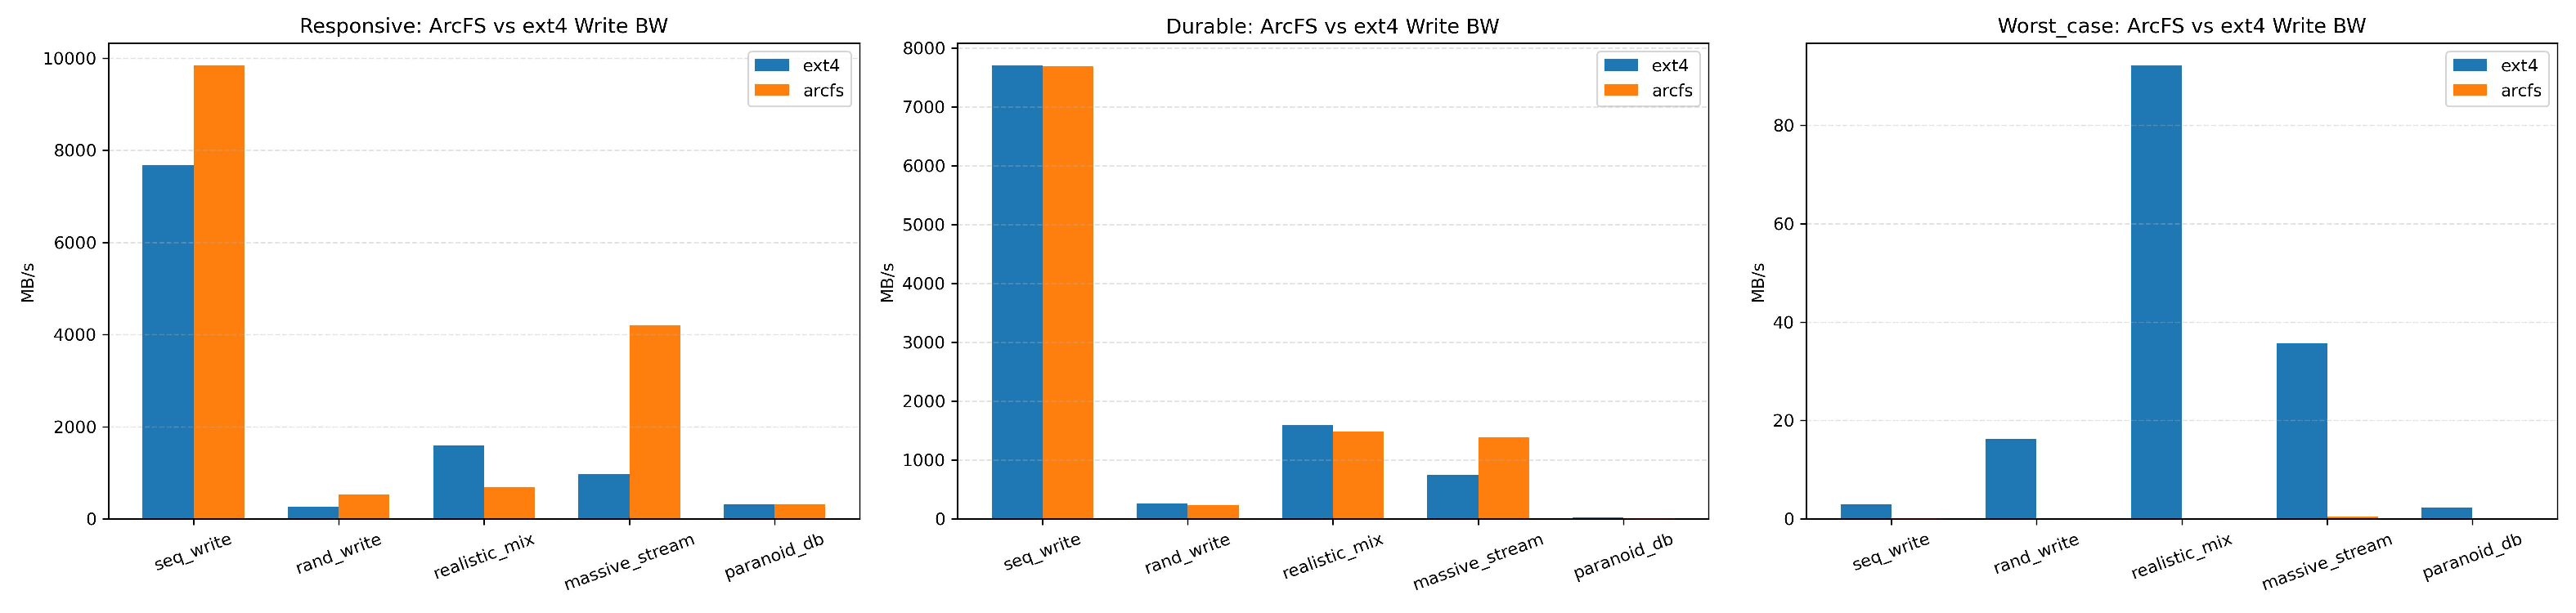
\includegraphics[width=\columnwidth]{fig1}
\caption{ArcFS write bandwidth relative to ext4 across the responsive
  (left) and durable (right) evaluation classes. ArcFS outperforms ext4
  by up to $9.2\times$ in the responsive class; the gap narrows under
  durable fsync constraints, confirming that write-back buffering explains
  the responsive advantage.}
\label{fig:class_compare}
\end{figure}

\begin{table}[t]
\caption{Per-Profile Throughput Summary (R = Responsive, D = Durable)}
\label{tab:perf}
\centering
\renewcommand{\arraystretch}{1.2}
\footnotesize
\begin{tabular}{lrrrr}
\toprule
\textbf{Profile} & \textbf{ext4 R} & \textbf{ArcFS R} & \textbf{ext4 D} & \textbf{ArcFS D} \\
\midrule
\texttt{seq\_write}      & 463\,MB/s  & 4,276\,MB/s & \multicolumn{2}{c}{near-parity} \\
\texttt{rand\_write}     & 68K\,IOPS  & 135K\,IOPS  & 68K\,IOPS & 60K\,IOPS \\
\texttt{massive\_stream} & 971\,MB/s  & 4,200\,MB/s & 746\,MB/s  & 1,383\,MB/s \\
\texttt{realistic\_mix}  & 29K\,IOPS  & 12K\,IOPS   & 29K\,IOPS & 27K\,IOPS \\
\texttt{paranoid\_db}    & 80K\,IOPS  & 83K\,IOPS   & 1.45\,MB/s & 3.48\,MB/s \\
\bottomrule
\end{tabular}
\end{table}

Figure~\ref{fig:class_compare} shows the aggregate class-level comparison;
Table~\ref{tab:perf} details per-profile results.
In the \textbf{responsive} class, ArcFS achieves 4,276\,MB/s sequential
write throughput, outperforming ext4 (463\,MB/s) by 9.2$\times$.  The
mechanism: the FUSE write handler performs an O(1) cache lookup, marks the
entry dirty, and returns---no disk I/O occurs until eviction, \texttt{fsync},
or close.  Under random 4\,KB pressure, ArcFS sustained 135K\,IOPS
(vs.\ 68K for ext4) at 0.009\,ms mean latency.

In the \textbf{durable} class, enforcing \texttt{fsync} semantics removes
the buffering advantage and throughput converges toward physical disk limits,
confirming that the responsive-class numbers reflect genuine I/O coalescing.
The notable exception is \texttt{paranoid\_db} (one \texttt{fsync} per 4\,KB
write): ArcFS achieves 3.48\,MB/s versus ext4 at 1.45\,MB/s, demonstrating
that the metadata-store commit path handles high-frequency sync points without
blocking.  All other durable profiles are near-parity with ext4.

\subsection{Integrity Verification}

\begin{figure}[t]
\centering
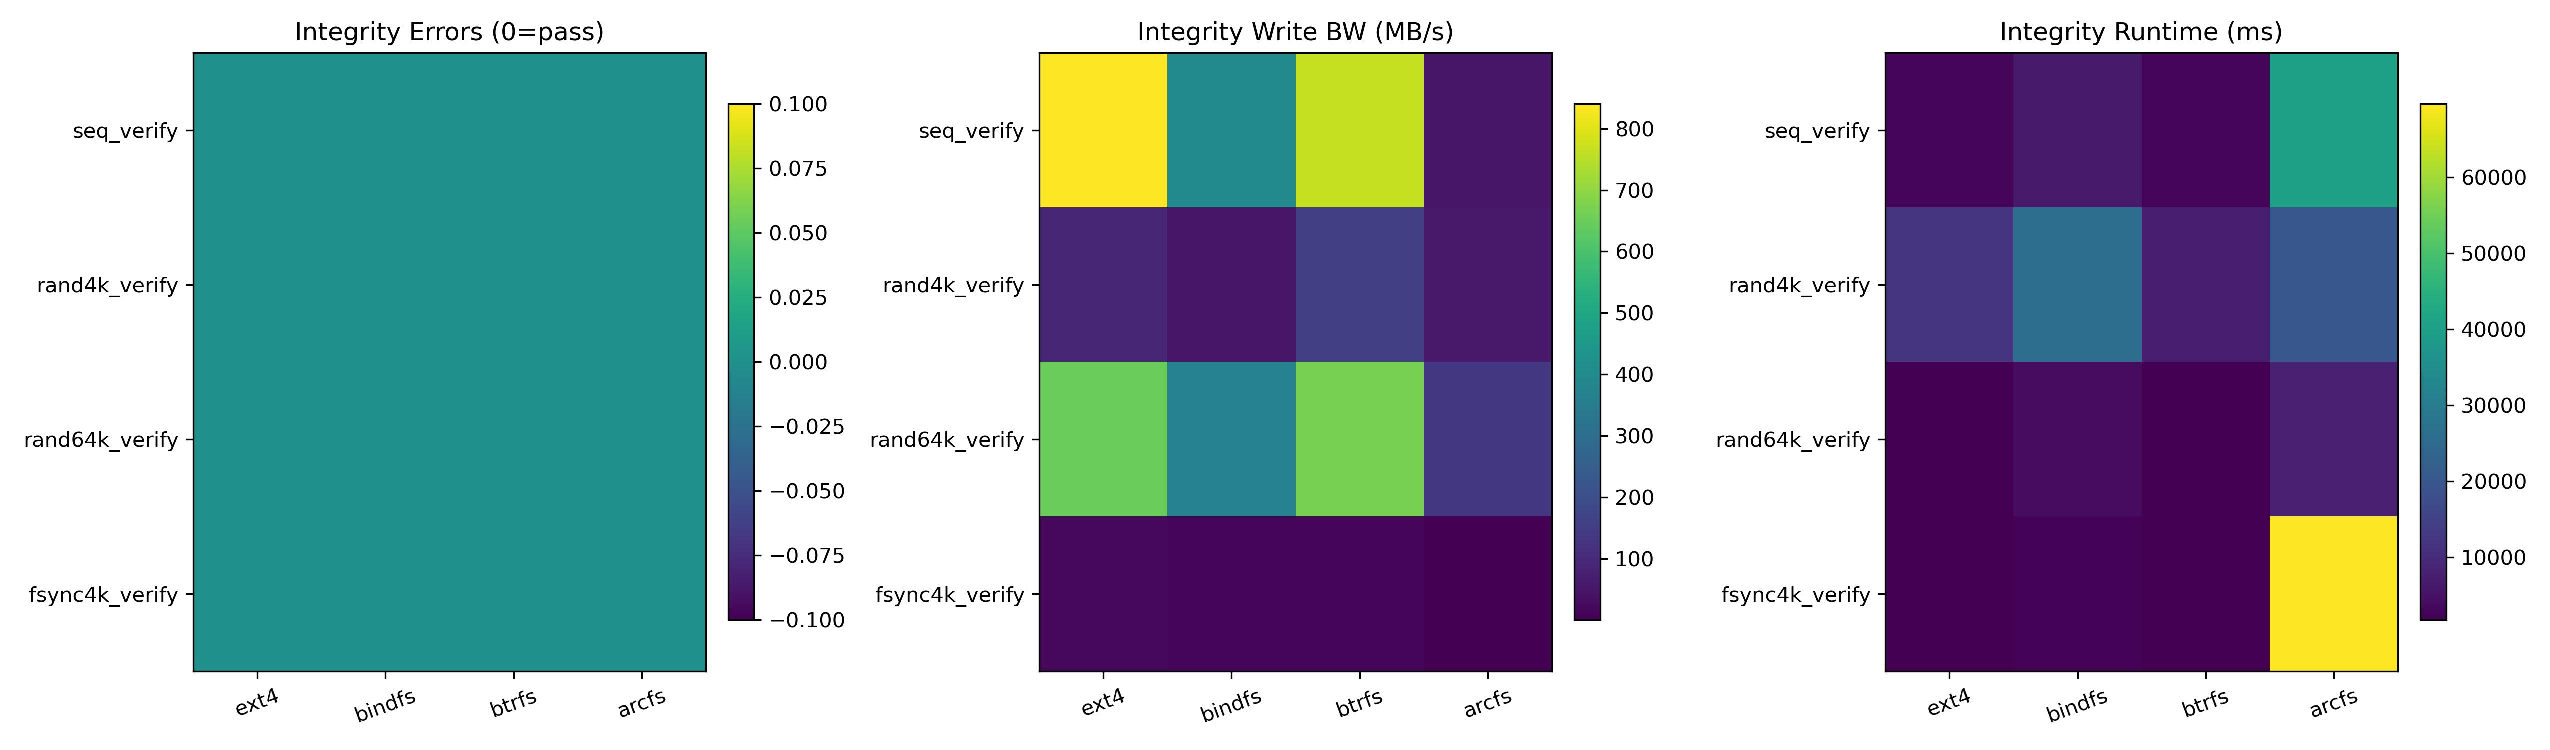
\includegraphics[width=\columnwidth]{fig2}
\caption{Integrity suite summary. All targets returned exit code 0
  (zero errors) across sequential, random 4\,KB, and random 64\,KB
  verification profiles. ArcFS shows higher wall-clock runtime on
  \texttt{fsync4k\_verify} due to user-space flush cost per sync point,
  a structural property of the FUSE architecture.}
\label{fig:integrity}
\end{figure}

CRC32c verify jobs write deterministic data and re-read it with the cache
purged; ArcFS returned zero errors across all three profiles
(\texttt{seq\_verify}, \texttt{rand4k\_verify}, \texttt{rand64k\_verify}),
confirming lossless round-trips through the full chunking and decompression
pipeline (Figure~\ref{fig:integrity}).  Higher wall-clock runtime on
\texttt{fsync4k\_verify} is architectural: each 4\,KB cycle crosses the
FUSE boundary, chunking, CAS lookup, and decompression; correctness is not
affected.

\subsection{Deduplication Efficiency}

\begin{figure}[t]
\centering
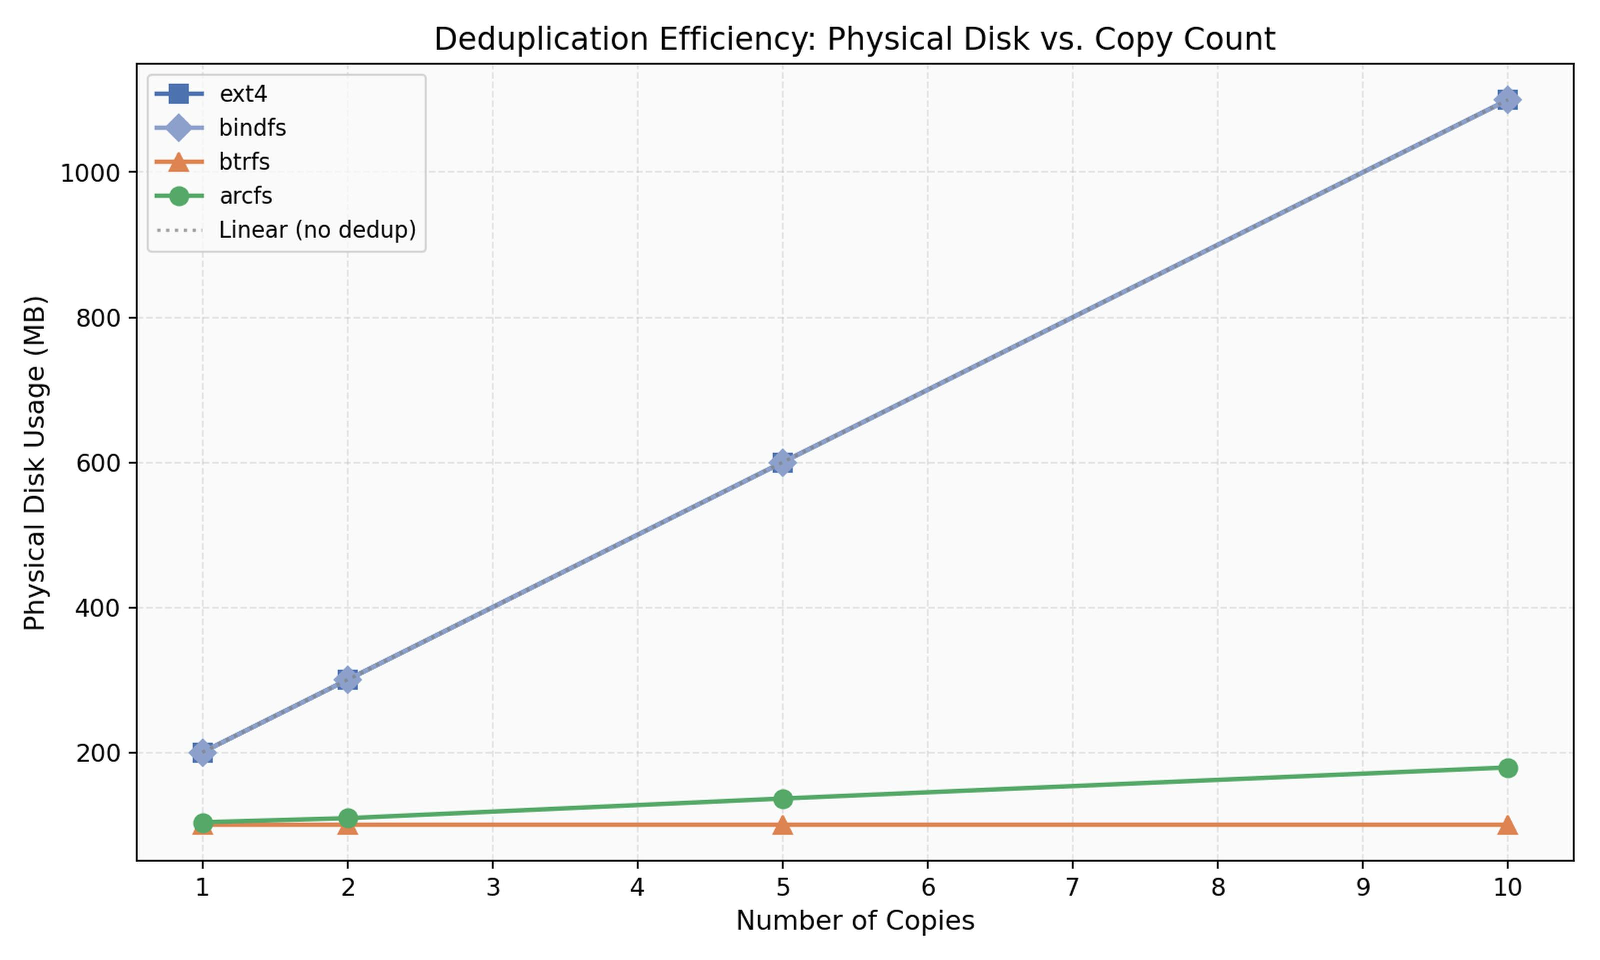
\includegraphics[width=\columnwidth]{fig3}
\caption{Physical disk consumption versus copy count for a 100\,MB
  reference file. Ext4 and bindfs grow strictly linearly. Btrfs stays
  constant at $\sim$21\,MB via O(1) kernel reflink. ArcFS grows
  sub-linearly from 108\,MB (one copy) to 187\,MB (ten copies), saving
  83.7\% of the 1,153\,MB logical total.}
\label{fig:dedup}
\end{figure}

Figure~\ref{fig:dedup} measures inline deduplication. At ten identical
copies of a 100\,MB reference file, ext4 and bindfs consume the full
1,153\,MB logical total. Btrfs maintains a constant $\sim$21\,MB
footprint through kernel-level reflink clones. ArcFS grows from 108\,MB
to 187\,MB, achieving 83.7\% space savings.  The 8\,MB overhead per
additional copy arises from per-inode metadata and recipe entries,
directory edge records, and minor chunk boundary variation from the Gear-hash rolling window at
file start (the chunker is re-initialized for each copy; the first chunk
of each copy begins at hash $h = 0$, which converges to the same boundary
pattern after a few hundred bytes, so deduplication efficiency for body
chunks is near-100\%).

All deduplication occurs transparently during ingestion via
\texttt{write\_chunk()}'s existence check; no offline dedup pass or
explicit reflink call is required.

\subsection{Compression Efficiency}

\begin{figure}[t]
\centering
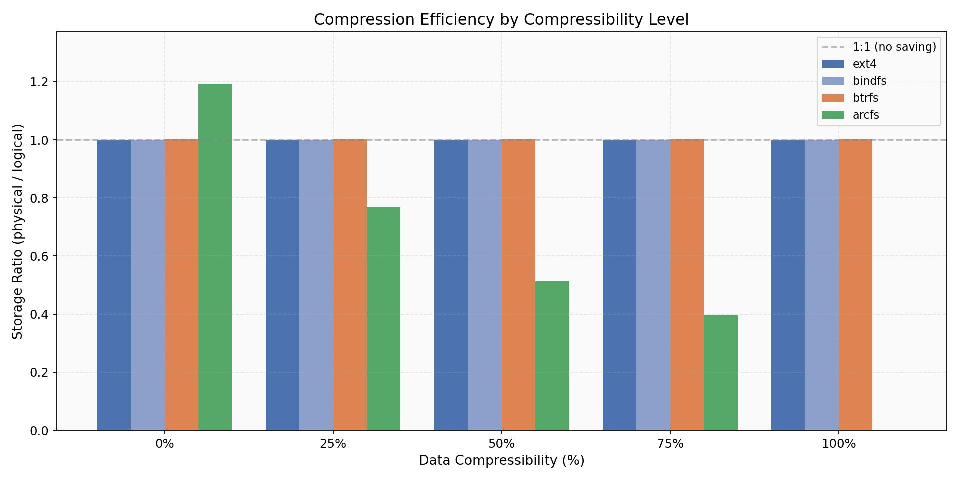
\includegraphics[width=\columnwidth]{fig4}
\caption{Physical-to-logical storage ratio versus data compressibility
  (0\% = pure random bytes; 100\% = uniform zeros). Ext4, bindfs, and
  uncompressed Btrfs hold a 1.0 ratio at all levels. ArcFS achieves
  0.77 at 25\%, 0.51 at 50\%, and 0.396 at 75\% compressibility.
  Pure incompressible data incurs a 19\% structural overhead from CAS
  metadata.}
\label{fig:compress}
\end{figure}

Figure~\ref{fig:compress} sweeps compressibility from 0\% (random bytes)
to 100\% (uniform zeros). ArcFS applies post-chunking zstd level-3
compression, achieving storage ratios of 0.77 at 25\% compressibility,
0.51 at 50\%, and 0.396 at 75\%. At 100\% compressibility, the ratio
falls to 0.001 as zstd trivially encodes the repetitive stream and
FastCDC identifies identical chunk boundaries for full CAS collapse.

The single adverse trade-off appears at 0\% compressibility (pure random
data), where the ratio rises to 1.19, a 19\% structural overhead. zstd
framing headers, SHA-256 hashes stored in metadata recipe entries, and
the two-level CAS directory structure account for this penalty. Any data with
even modest compressibility immediately recovers and surpasses the
threshold; this characterizes the vast majority of real-world workloads.

\subsection{Snapshot Storage Cost}

\begin{figure}[t]
\centering
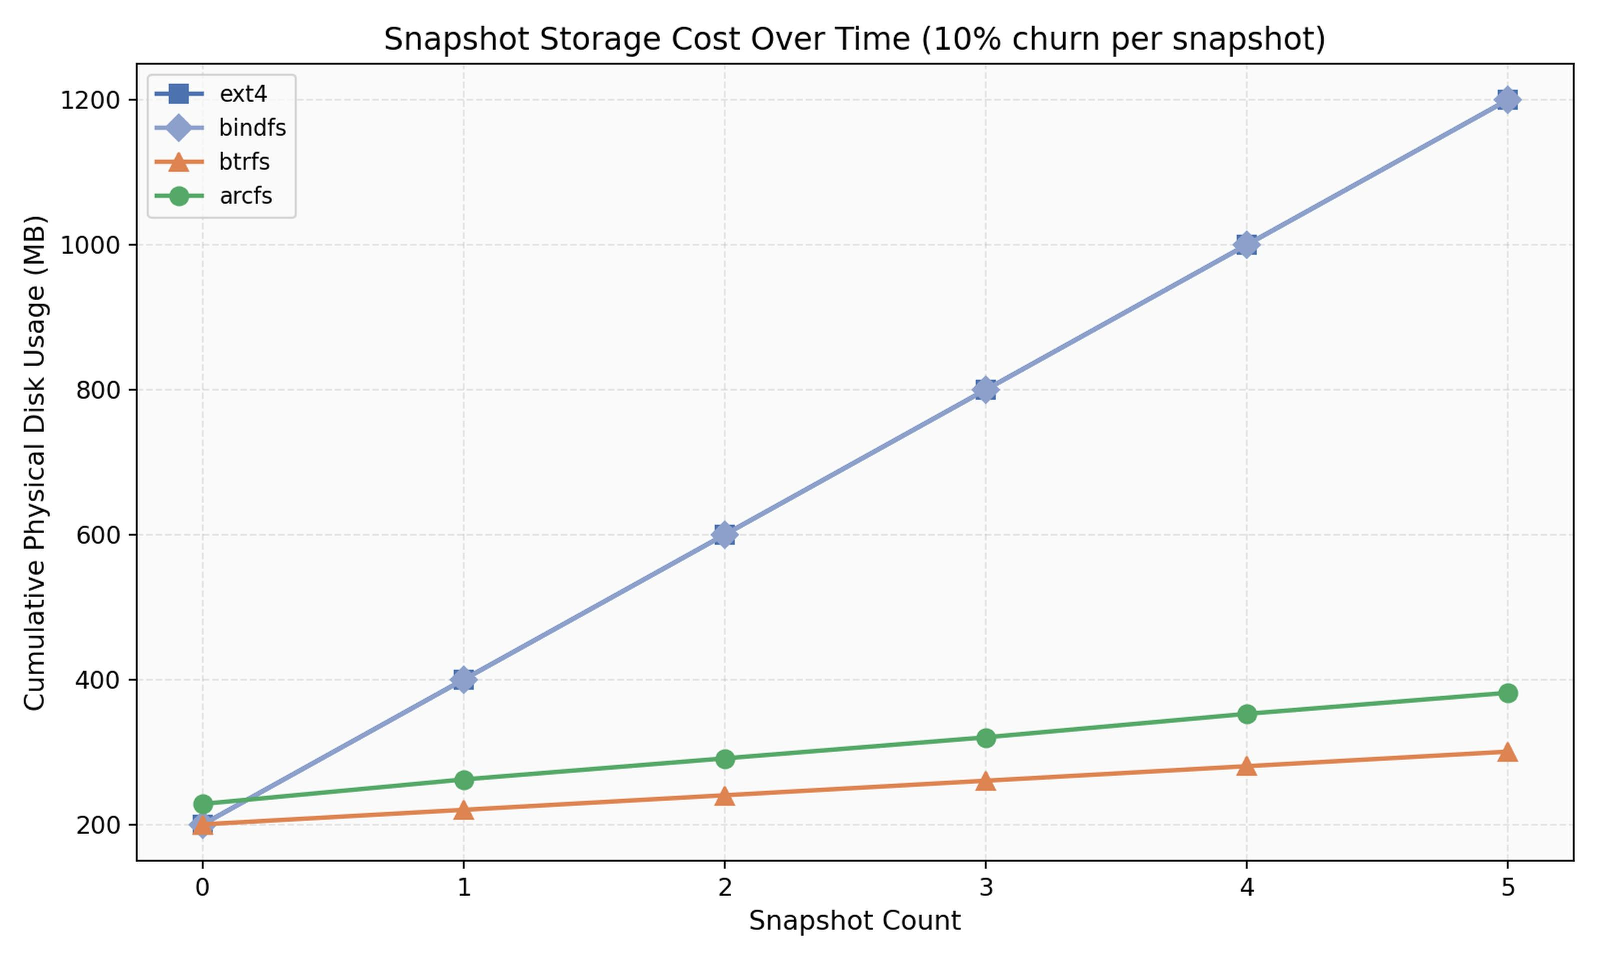
\includegraphics[width=\columnwidth]{fig5}
\caption{Cumulative physical disk usage across five successive snapshots
  with 10\% data churn per snapshot (200\,MB base). Ext4 and bindfs
  grow by $\sim$209\,MB per snapshot (full copy). Btrfs grows by
  $\sim$21\,MB (kernel CoW extent sharing). ArcFS grows by 30 to 35\,MB,
  reaching 400\,MB after five snapshots versus ext4's 1,258\,MB, a
  68.2\% reduction.}
\label{fig:snapshot}
\end{figure}

Figure~\ref{fig:snapshot} tracks cumulative disk usage across five
successive snapshots with 10\% data modification between each pair on
a 200\,MB base. Ext4 and bindfs copy the full base on each snapshot,
reaching 1,258\,MB after five versions. Btrfs grows by $\sim$21\,MB per
snapshot (matching the 10\% churn rate) through kernel-level CoW extent
sharing. ArcFS grows by 30 to 35\,MB per snapshot, reaching 400\,MB
(a 68.2\% storage reduction versus ext4).

The $\sim$10\,MB incremental cost above Btrfs reflects two factors.
First, the snapshot clone writes new inode metadata and recipe entries for
every inode, adding metadata overhead proportional to inode count rather
than churn size. Second,
FastCDC's content-defined boundaries occasionally split modified regions
differently at modification edges, producing a small number of new unique
chunks adjacent to the 10\% churn boundary.  The combined effect of
pointer-based CAS sharing and zstd compression delivers snapshot
efficiency closely approaching kernel-native CoW from user space.

\subsection{Mixed Realistic Workload}

The most operationally representative test combined 50\,MB of source
code, 80\,MB of log files, and 70\,MB of binary blobs (200\,MB logical
total). Ext4 and bindfs consumed $\sim$225\,MB. Btrfs without
transparent compression consumed 234\,MB. ArcFS consumed 96.3\,MB,
57.6\% less than ext4. FastCDC identified shared segments across similar
source files; SHA-256 CAS deduplicated those chunks; and zstd level-3
substantially compressed the highly repetitive log segments. Of the filesystems evaluated, ArcFS alone combines CDC deduplication,
per-chunk compression, and CoW versioning in a single transparent write
path.  Figure~\ref{fig:heatmap} consolidates all four disk-usage profiles;
ArcFS achieves the lowest physical-to-logical ratio on mixed workloads (0.07)
while Btrfs dominates on pure deduplication (0.016) via O(1) reflink.

\begin{figure}[t]
\centering
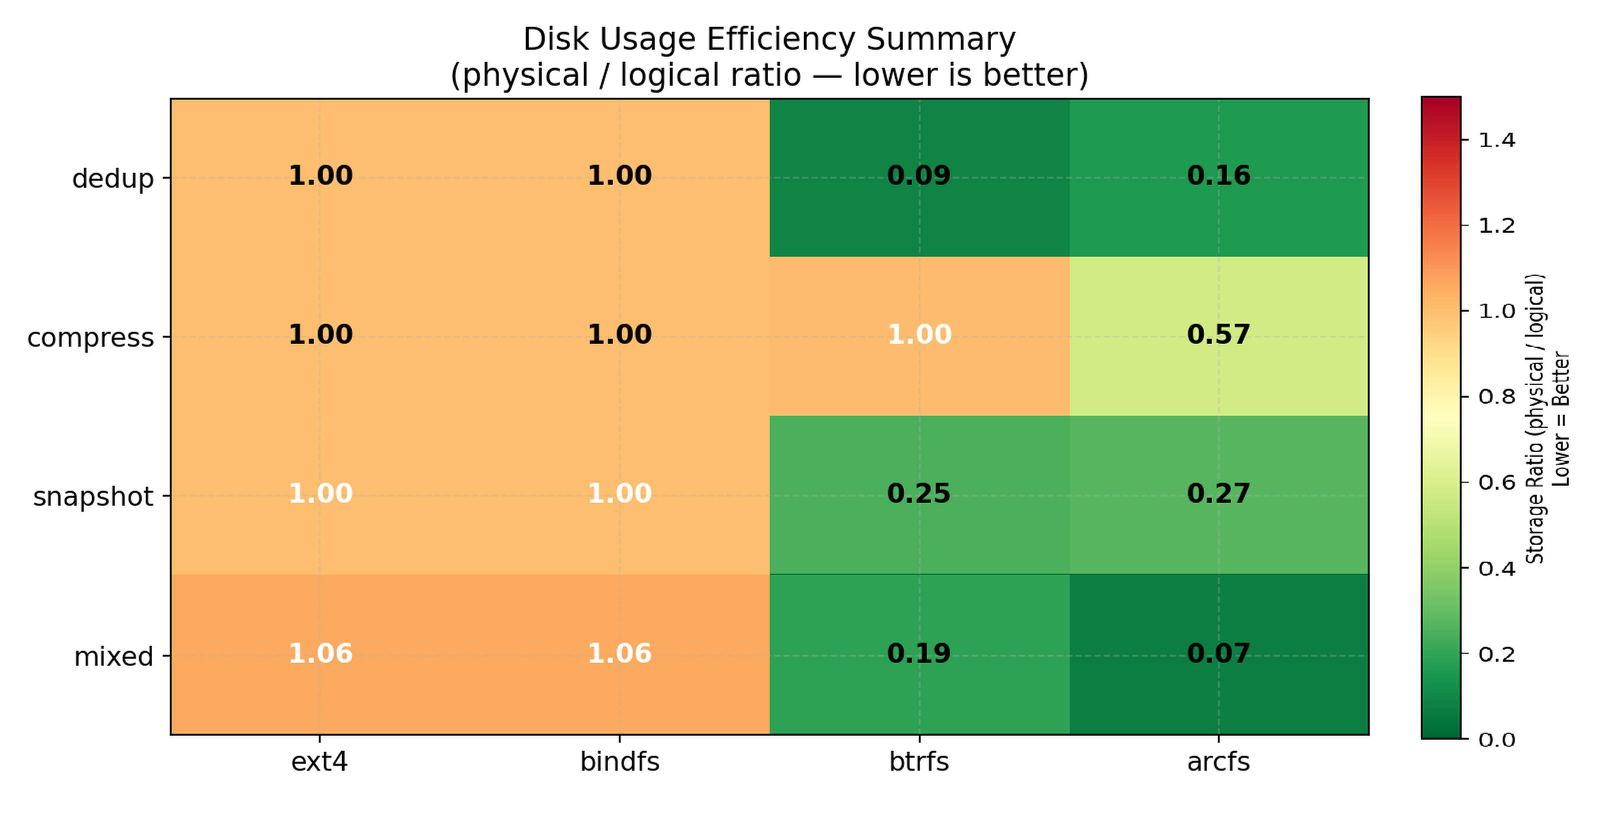
\includegraphics[width=\columnwidth]{fig6}
\caption{Disk usage efficiency heatmap (physical/logical ratio, lower is
  better). ArcFS leads on mixed and compression workloads; Btrfs leads on
  pure deduplication via kernel reflink.}
\label{fig:heatmap}
\end{figure}

%% ─────────────────────────────────────────────────────────────────────────────
\section{Discussion}

\subsection{Two-Class Performance Trade-off}

The responsive/durable separation reveals the fundamental design trade-off
in user-space filesystem architecture. In the responsive class, the
write-back LRU cache transforms a pipeline with four sequential CPU-bound
stages (FastCDC, SHA-256, zstd, metadata commit) into a single in-memory
buffer update, raising effective throughput by an order of magnitude.
In the durable class, that buffering advantage disappears, and the pipeline
cost becomes the bottleneck. ArcFS remains competitive with kernel
filesystems in the durable class on most profiles, which confirms that the
four-stage pipeline does not introduce catastrophic overhead, only a
predictable latency proportional to per-write flush cost.

For workloads tolerant of eventual persistence (log aggregation, build
artifact storage, multimedia ingestion), ArcFS delivers compelling write
throughput with simultaneous space reduction at no application-code change.
For workloads demanding synchronous durability (database write-ahead logs,
transactional record systems), ArcFS provides correct behavior with
throughput near kernel baselines but not exceeding them.

\subsection{Overhead Sources and Limits}

Three overheads characterize ArcFS relative to kernel filesystems. First,
every FUSE request crosses the kernel/user boundary twice, adding latency
that accumulates on metadata-intensive workloads such as random 4\,KB reads
with cache misses. Second, the FastCDC pipeline introduces measurable CPU
work per flush: Gear-hash evaluation across the byte stream, SHA-256 digest
computation, zstd framing, and metadata transaction commit all execute
synchronously in the daemon. Third, pure incompressible data incurs a 19\%
storage overhead from CAS metadata structures, representing the worst-case
structural penalty.

The O($n$) scan in the LRU promotion step deserves attention under
high-ingest workloads. Each write call that triggers cache entry promotion
scans up to 1,024 inode IDs in the LRU queue.  For a workload that
writes to 1,024 distinct inodes in rapid succession, the LRU maintenance
cost approaches $1{,}024^2 / 2$ comparisons per eviction cycle---roughly
500,000 comparisons---which at a few nanoseconds each contributes
measurably to per-write latency.  Replacing the linear-scan queue with a
doubly-linked list and a companion hash map of node positions would reduce
LRU maintenance to O(1) and is a natural implementation improvement.

Two additional overheads merit disclosure for cloud deployment contexts.
First, the chunk-read path does not re-verify the SHA-256 hash of the
decompressed payload; the system relies on the host filesystem's
block-level integrity guarantees.  Silent bit-rot in the CAS blobs
would produce incorrect data without detection.  Second, CAS blobs are
stored as plain files on the host filesystem; any process with read
access to the storage directory can observe chunk content directly.
For multi-tenant deployments, per-chunk encryption (e.g., AES-GCM keyed
from the chunk hash and a tenant secret) is necessary to prevent
cross-tenant data observation through the hash oracle.

\subsection{Comparison with Prior Systems}

ArcFS occupies a design point approached only partially by prior work.
LBFS~\cite{muthitacharoen2001lbfs} performs CDC deduplication but at the
network layer, with no tag-based access or versioning.
BorgBackup~\cite{borgbackup2024} provides application-level CDC
deduplication with encryption, but requires all writers to route through
the same agent. BetrFS~\cite{jannen2015betrfs} achieves write-optimized
metadata with B\textsuperscript{$\varepsilon$}-trees but does not integrate
content deduplication or semantic tagging. The Bento
system~\cite{miller2021bento} eliminates FUSE context-switch overhead
through Rust-based in-kernel modules but does not integrate deduplication
or semantic tagging.

WiscKey~\cite{lu2017wisckey} achieves a key-value separation analogous to
ArcFS's split between sled recipe keys and CAS blob values, but operates
as a storage engine rather than a filesystem interface.  CephFS
serves as a distributed filesystem reference~\cite{weil2006ceph}: it scales
metadata across multiple MDS daemons, a capability that would require
distributing ArcFS's metadata store across nodes.

Venti~\cite{quinlan2002venti} is the closest architectural ancestor: it
stores write-once, content-addressed blocks identified by SHA-1 hashes,
and serves them over a network protocol.  ArcFS extends the Venti model
with variable-size chunking (rather than fixed-size blocks), zstd
compression, CoW versioning, and a POSIX namespace layer with virtual
tag-based navigation.

%% ─────────────────────────────────────────────────────────────────────────────
\section{Limitations and Future Work}
\label{sec:limits}

The following limitations are grounded in the current implementation;
each entry states the impact, root cause, and remediation path.

\paragraph{L1 — Offline GC with unsafe concurrent-use window.}
Running the garbage collector concurrently with a mounted filesystem
risks deleting a CAS blob written between the mark and sweep phases,
causing an I/O error on the next access to that inode.  \textit{Root cause}:
no coordination protocol exists between the CLI GC and a running mount.
\textit{Remedy}: an epoch counter incremented on each write; GC
re-validates hashes that appeared after Phase~1's epoch before deleting.

\paragraph{L2 — O(n) LRU update.}
The LRU promotion step linearly scans up to 1,024 entries on every write;
overhead is negligible at 4\,KB but dominates at very small write sizes.
\textit{Root cause}: the linear-scan queue structure has no O(1) position
lookup.  \textit{Remedy}: doubly-linked list with a companion hash map for
O(1) promote and evict.

\paragraph{L3 — Snapshot recipe leak.}
Snapshot deletion removes only the top-level snapshot record; the
O($n_i$) cloned inode metadata and recipe entries persist indefinitely,
and GC treats them as live.  Unreclaimable storage grows as
$O(S \cdot k_s)$ for $S$ deleted snapshots each with $k_s$ unique chunks.
\textit{Remedy}: cascade-delete all reachable inode entries when a
snapshot is removed.

\paragraph{L4 — No on-read hash verification.}
Silent bit-rot in a CAS blob returns corrupt data without any signal,
because the chunk-read path does not re-hash the decompressed payload.
\textit{Remedy}: an optional \texttt{--verify-reads} flag that returns
an I/O error on SHA-256 mismatch.

\paragraph{L5 — No encryption; hash-oracle leakage.}
CAS blobs are plain files; any process with storage-directory access
can read chunk content, and the presence of a specific CAS path reveals
that a given SHA-256 hash has been ingested.  \textit{Remedy}: per-chunk
AES-GCM with an HKDF-derived tenant key eliminates both attack vectors.

\paragraph{L6 — Unbounded GC active-set memory.}
Phase~1 materialises all referenced chunk hashes in RAM; at 64\,B per
hex string, a 400\,GB dataset ($\sim$100M chunks) requires $\sim$6.4\,GB
resident GC memory.  \textit{Remedy}: a merge-scan that sorts both the
metadata scan and the CAS walk by hash, deleting orphans without full
materialisation.

\paragraph{L7 — Single-threaded FUSE dispatch.}
The FUSE daemon serialises all requests on one thread, capping
multi-writer throughput regardless of core count; all benchmarks in this
paper are single-writer.  \textit{Remedy}: multi-threaded FUSE mount with
concurrent-safe data structures.

\paragraph{L8 — Single-node metadata and CAS.}
Both the metadata store and the CAS directory are local to the daemon
process and cannot scale beyond one host.  \textit{Remedy}: replace the
metadata store with TiKV/FoundationDB and the CAS directory with an
S3-compatible object store~\cite{weil2006ceph}.

\paragraph{L9 — Read path not benchmarked.}
Cache-hit throughput and cold-cache random-read latency are
uncharacterised; both are deferred to a follow-on evaluation.

\paragraph{L10 — Metadata orphaning on unlink.}
File deletion removes only the directory-entry edge; the inode's metadata
and recipe records along with their referenced CAS blobs are never
reclaimed by GC.  \textit{Remedy}: cascade-delete inode metadata on
deletion or add a background metadata sweeper.

\paragraph{L11 — Real/virtual inode range not enforced.}
The real inode counter is not prevented from crossing the virtual inode
range boundary (1,000,000), risking ID collisions with TagFS virtual
inodes at large inode counts.  \textit{Remedy}: enforce a hard upper
bound for real inodes or move virtual inodes to a disjoint high-bit range.

%% ─────────────────────────────────────────────────────────────────────────────
\section{Conclusion}

ArcFS demonstrates that a single Rust FUSE daemon can integrate
content-defined chunking, content-addressable storage, copy-on-write
versioning, and tag-based semantic navigation without sacrificing POSIX
compatibility or data correctness.

The write-back LRU cache coalesces writes entirely in memory and delivers
9.2$\times$ sequential write throughput over ext4 in the responsive class.
The FastCDC chunking engine maintains per-file hash isolation by allocating
a fresh state instance per ingestion, structurally preventing cross-file
boundary interference.
The offline garbage collector operates in two phases: a metadata scan
that builds the active chunk set, followed by a CAS directory walk that
deletes orphaned blobs.  On storage efficiency, ArcFS
achieves 83.7\% deduplication savings on identical files, reduces
mixed-workload disk consumption by 57.6\% over ext4, and holds snapshot
storage costs within 1.3$\times$ of kernel-native Btrfs. All CRC32c
integrity verifications pass at zero error rate, confirming lossless
reconstruction through the full chunking and decompression pipeline.

Eleven quantified limitations (L1--L11) provide a concrete development
roadmap; addressing L7 (multi-threaded dispatch) and
L8 (distributed metadata and CAS backends) would position ArcFS as a
practical cloud storage primitive---a transparent deduplication and
semantic-navigation gateway over distributed object stores---deployable
without modification to existing applications.

%% ─────────────────────────────────────────────────────────────────────────────
\section*{Acknowledgements}

The authors thank the faculty and staff of the Department of Computer
Science and Engineering, PSG College of Technology, for access to
computing infrastructure used in benchmark execution.

%% ─────────────────────────────────────────────────────────────────────────────
\section*{CRediT authorship contribution statement}

\textbf{Kishoreadhith V:} Conceptualization, Software, Methodology,
Writing -- original draft, Visualization.
\textbf{Dhakkshin S R:} Software, Validation, Data curation.
\textbf{Anandkumar N S:} Conceptualization, Software, Writing --
review \& editing.
\textbf{M Raj Ragavender:} Software, Validation, Data curation.
\textbf{Rithvik K:} Software, Validation.
\textbf{Dr.\ Arulanand N:} Supervision, Writing -- review \& editing,
Resources, Project administration.

%% ─────────────────────────────────────────────────────────────────────────────
\section*{Declaration of competing interests}

The authors declare that they have no known competing financial interests
or personal relationships that could have appeared to influence the work
reported in this paper.

%% ─────────────────────────────────────────────────────────────────────────────
\section*{Funding}

This research did not receive any specific grant from funding agencies
in the public, commercial, or not-for-profit sectors.

%% ─────────────────────────────────────────────────────────────────────────────
\section*{Declaration of generative AI and AI-assisted technologies in
the manuscript preparation process}

During the preparation of this work the authors used Claude (Anthropic)
in order to assist with literature synthesis, \LaTeX{} formatting, and
prose editing. After using this tool, the authors reviewed and edited
the content as needed and take full responsibility for the content of
the published article.

%% ─────────────────────────────────────────────────────────────────────────────
\section*{Data availability}

The source code for ArcFS is publicly available at
\url{https://github.com/kishoreadhith-v/arcfs}.

%% ─────────────────────────────────────────────────────────────────────────────
\bibliographystyle{elsarticle-num}
\bibliography{references}

\end{document}
